%%
%% Author: Jordan Osborn
%% 01/01/2019
%%

% Preamble
\documentclass[11pt]{article}

% Packages
\usepackage{amsmath, mathrsfs}
\usepackage{titling}
\usepackage{hyperref}
\usepackage[sorting=none, backend=bibtex]{biblatex}
\usepackage{graphicx}
\usepackage{float}
\usepackage{enumitem}

\addbibresource{report.bib}

\title{A new video analysis algorithm for the study of crowd dynamics}
\author{Jordan Osborn (jo357) Supervisor: Professor Pietro Cicuta (pc245)}
% Document
\begin{document}
\begin{titlingpage}
    \maketitle
\end{titlingpage}


\clearpage
\title{A new video analysis algorithm for the study of crowd dynamics}
\author{Supervisor: Professor Pietro Cicuta (pc245)}
\maketitle
\section*{Abstract}

\clearpage
\tableofcontents
% TODO: 5000 Words 

\clearpage
\section{Introduction}
%TODO: Tuesday 16/04
In this project the technique of Differential Dynamic Microscopy will be applied to videos of crowd motion. This technique provides information about the dynamical behaviour of objects in a video without the use of image segmentation. DDM was first carried out in 2008, to analyse the dynamics of colloidal particles in Brownian motion \cite{ddm0}. A video of colloidal particles will be analysed and will act as a test case for the code developed in this project. Differential Dynamic Microscopy has primarily been used to analyse the motion of microscopic particles \cite{ddm1} \cite{ddm2}. This project was undertaken in order to determine the applicability of DDM to macroscopic motion i.e. crowd motion videos. A literature review will be carried out in section 2, but this will mainly be centred around the microscopic applications of DDM as prior literature is not available for the application of DDM to macroscopic motion. The code developed as a part of this project is intended to act as a reference for further development (e.g. for real time commercial crowd analysis) and so has been developed with execution speed as well as accuracy as a priority. Certain design decision were undertaken to achieve this. Further discussion about implementation will be carried out in section 3.
\\\\
DDM is used to extract dynamical information from videos by analysing the Intensity profile (in k-space) of the differences between a starting frame and lagging frames. This intensity is a function of wave-vector q and $\tau$ the time delay between frames. By fitting this curve to the expected image structure function we can extract dynamical information about the system. A detailed discussion of the theory behind DDM will occur in section 3. (The information extractable from a DDM analysis is sensitive to the particular dynamics of the system for example for particles undergoing Brownian motion it is possible to extract the size of the diffusing particle\cite{ddm1}.)
\\\\
There are two primary types of DDM analysis. Single-scale DDM and multi-scale DDM. Single-scale DDM performs DDM analysis on the entire image and so picks up a combination of the spatial and temporal scales of synchronisation \cite{ddm2}. Where as Multi-scale DDM performs DDM analysis on individual tilings of the image from a full-scale image down to the smallest tile size (determines the mini-mum wave-vector that can be compared across tiles)\cite{ddm2}. In this way spatial and temporal scales of synchronisation can be picked up separately. A more in-depth description of the two methods will take place in sections 3 and 4.  
\\\\
Each type of analysis will yield different pieces of dynamical information. Both methods will be run on a large database of approximately 400 videos\cite{crowdMotionDB}. The data will then be analysed, dynamical information will be extracted and then compared to that extractable by eye (for select videos). This analysis and discussion will take place in sections 5 and 6.
\\\\
DDM has the potential to be used to implement real-time analysis of crowd motion without the use of image segmentation, or the use of machine learning (expensive datasets and long training periods). Section 7 contains an in depth discussion about the future of DDM as applied to the analysis of crowd motion. The hope is that DDM might one day be used to help implement real-time crowd safety/monitoring systems in environments such as public transportation, stadiums, city centres etc.

\clearpage
\section{Literature Review}
%TODO: Sunday 21 / 04 / 19

\clearpage
\section{Theory}

DDM or Differential Dynamic Microscopy is a method that can be used to analyse an image sequence by taking a difference between two images (removes static features and retains only motion/differences between frames), and then taking the 2D spatial Fourier transform (using a 2D FFT algorithm\cite{fft}) of this difference to obtain an image structure function.
From this function many properties of the motion can be determined.\cite{ddm1}
An outline of the mathematics is given below:

\begin{equation}
    d(\textbf{r}, t_0, \tau) = I(\mathbf{r}, t_0 + \tau) - I(\mathbf{r}, t_0)
\end{equation}
The function $\textit{I}$ encodes the 2D projection of the scene along the optical axis of the camera (i.e the image intensity) as a function of position and of time.
This intensity could well be in colour (tuple of 3 intensities for red, green and blue) or could be in greyscale. Colour information may provide extra information about motion but may also be an artefact produced by lighting effects. Greyscale images would provide the necessary motion information and would not be vulnerable to the issues colour images may pose (more computational complexity, does a colour change really indicate motion etc.)

\begin{equation}
    \mathscr{F} (d(\textbf{r}, t_0, \tau) ) = \mathscr{F} (I(\mathbf{r}, t_0 + \tau) - I(\mathbf{r}, t_0)) = \mathscr{F}(I(\mathbf{r}, t_0 + \tau)) - \mathscr{F}(I(\mathbf{r}, t_0))
\end{equation}

The second equality results from the linearity of the Fourier transform and reduces computational complexity as it allows you to cache Fourier transforms at each time and then compute their difference.
This reduces the number of Fourier transforms you need to compute, hence provides a computational optimisation.\cite{ddm2}
We now have

\begin{equation}
    d(\textbf{q}, t_0, \tau) ) = \mathscr{F}(I(\mathbf{r}, t_0 + \tau)) - \mathscr{F}(I(\mathbf{r}, t_0))
\end{equation}

Where $\textbf{q}$ is the 2D wave vector $(q_x, q_y)$.
Simplifications can be made if you can make some assumptions about the properties of the image, including isotropy and that motion is indifferent about the reference time (can average for all $t_0$).\cite{ddm1}
\\\\
The wave-vectors can be used to derive a wavelength $(\lambda = \frac{2\pi}{|\textbf{q}|})$ which gives you the length scale probed by a particular mode.
Information about the system's dynamics can be obtained by looking at how the amplitudes of the Fourier modes for each q changes with the time differences between frames $\tau$.\cite{ddm2}
\\\\

It has been shown in general that the image structure function takes the form given below \cite{ddm1}.
\begin{equation}
	I(\textbf{q}, \tau) = A(\textbf{q}) \cdot (1 - f(\textbf{q}, \tau)) + B(\textbf{q})
\end{equation}

Where $f(\textbf{q}, \tau)$ is the normalised "intermediate scattering function" as commonly measured in dynamic light scattering experiments \cite{DLSPecora}. A few analytical forms for f are known including Brownian motion and Ballistic motion \cite{DLSPecora}. The function f "characterises how quickly structure is lost over length scales ~ 1/q"\cite{ddm1}. The parameters A(\textbf{q}) and B(\textbf{q}) are functions related to the static scattering properties of the sample, to the details of the imaging process optics and to the noise in the acquisition \cite{ddm1}. These are just going to be considered as fitting parameters but some useful information can be extracted from them \cite{ddm1}. All interesting dynamical properties are often completely captured by $f(\textbf{q}, \tau)$ \cite{ddm1}. The intermediate scattering function f is the spatial Fourier transform of the Van-Hove self space-time correlation function \cite{DLSPecora}.

\begin{equation}
	f(\textbf{q}, \tau) = \mathscr{F} (G(\textbf{r}, \tau)) = \int d^3 \textbf{r} e^{i \textbf{q} \cdot \textbf{r}} G(\textbf{r}, \tau)
\end{equation}

The Van-Hove equation is the probability distribution for a particle with position $\textbf{R}_j(t)$ to suffer a displacement $\textbf{r}$ in a time $\tau$\cite{DLSPecora}.

\begin{equation}
	G(\textbf{r}, \tau) = \left\langle \delta (\textbf{r} - [\textbf{R}_j(t) - \textbf{R}_j(0)]) \right\rangle
\end{equation}

It is easy to see through the definitions above how dynamical information about the system can be extracted from the form of the intermediate scattering function.
\\\\
Now this is a complicated equation and so has only been solved analytically for a few cases. One of which is Brownian motion. In the case of Brownian motion the ISF has been shown to be

\begin{equation}
	f(\textbf{q}, \tau) = e^{- \tau / \tau_c(\textbf{q})} = e^{- \tau / (\frac{1}{D_T |\textbf{q}|^2})}
\end{equation}
where $D_T$ is the translational diffusion coefficient\cite{ddm1}. If we then fit this to data from videos behaving in a similar manner to Brownian motion we should then have $\tau_c$ as a function of $|\textbf{q}|$. Plotting this data on a log-log plot we should then see the characteristic form predicted by the equation above
\begin{equation}
\log{\tau_c} = -2 \cdot \log{|\textbf{q}|} - \log{D_T}
\end{equation}
By comparing the measured gradient to -2 we can see how valid the assumption of Brownian motion is. And from the y-intercept we can also derive a prediction for the translational diffusion coefficient $D_T$.
\\\\
Another solved case is that of Ballistic motion (isotropic motion). The form of the intermediate structure function in this case is 

\begin{equation}
	f(\textbf{q}, \tau) = sinc(|\textbf{q}| \cdot v \cdot \tau) \cdot e^{- \tau / \tau_c(\textbf{q})}
\end{equation} \cite{DLSPecora}.

Systems that show similar behaviour to ballistic motion should have a similar ISF, from the ISF we should therefore be able to extract the velocity of the crowd from the first peak in the intensity profile.
\\\\
A related method called multi-scale DDM (this project will make heavy use of this method) picks up temporal and spatial scales of synchronisation separately (normal single-scale DDM only picks up a combination).
In multi-scale DDM you perform a single-scale DDM over a whole series of different tilings of the image\cite{ddm1}. These tilings are chosen so that windows vary from a full scale image down to the smallest tile size (determines the minimum wave-vector that can be compared across tiles) (usually log spaced)\cite{ddm1}.
To reduce the number of tiles that need to be computed you can select only the tiles showing the most activity, an equation that can determine if a tile exceeds a threshold activity is
\begin{equation}
    \Sigma_{\textbf{r} \in tile} \sigma(\textbf{r}) = \Sigma_{\textbf{r} \in tile} \sqrt{\frac{\Sigma_{[t_0, t_0 + \tau]} (I(\mathbf{r}, t) - <I(\mathbf{r}, t)>)^2}{N - 1}} > \sigma_{threshold}
\end{equation}

Which sums all of the standard deviations (computed over the time period $\tau$) of the intensities at each position in the tile and then checks if this sum is greater than some threshold standard deviation.
If it is a valid inequality then that tile is said to be "active" otherwise it is "inactive".\cite{ddm2}
This is a very rudimentary activity classifying function.
There are other ways that a tile's activity can be classified which may need to be investigated.
\\\\
In the cross comparisons between the tiles of different sizes the scale of the collective motion should emerge.\cite{ddm1}
Other properties of the motion should emerge by studying how tau varies as a function of the wave-vector amplitude.\cite{ddm1}

\subsection{DDM example - Brownian motion}

\begin{figure}[H]
\centering
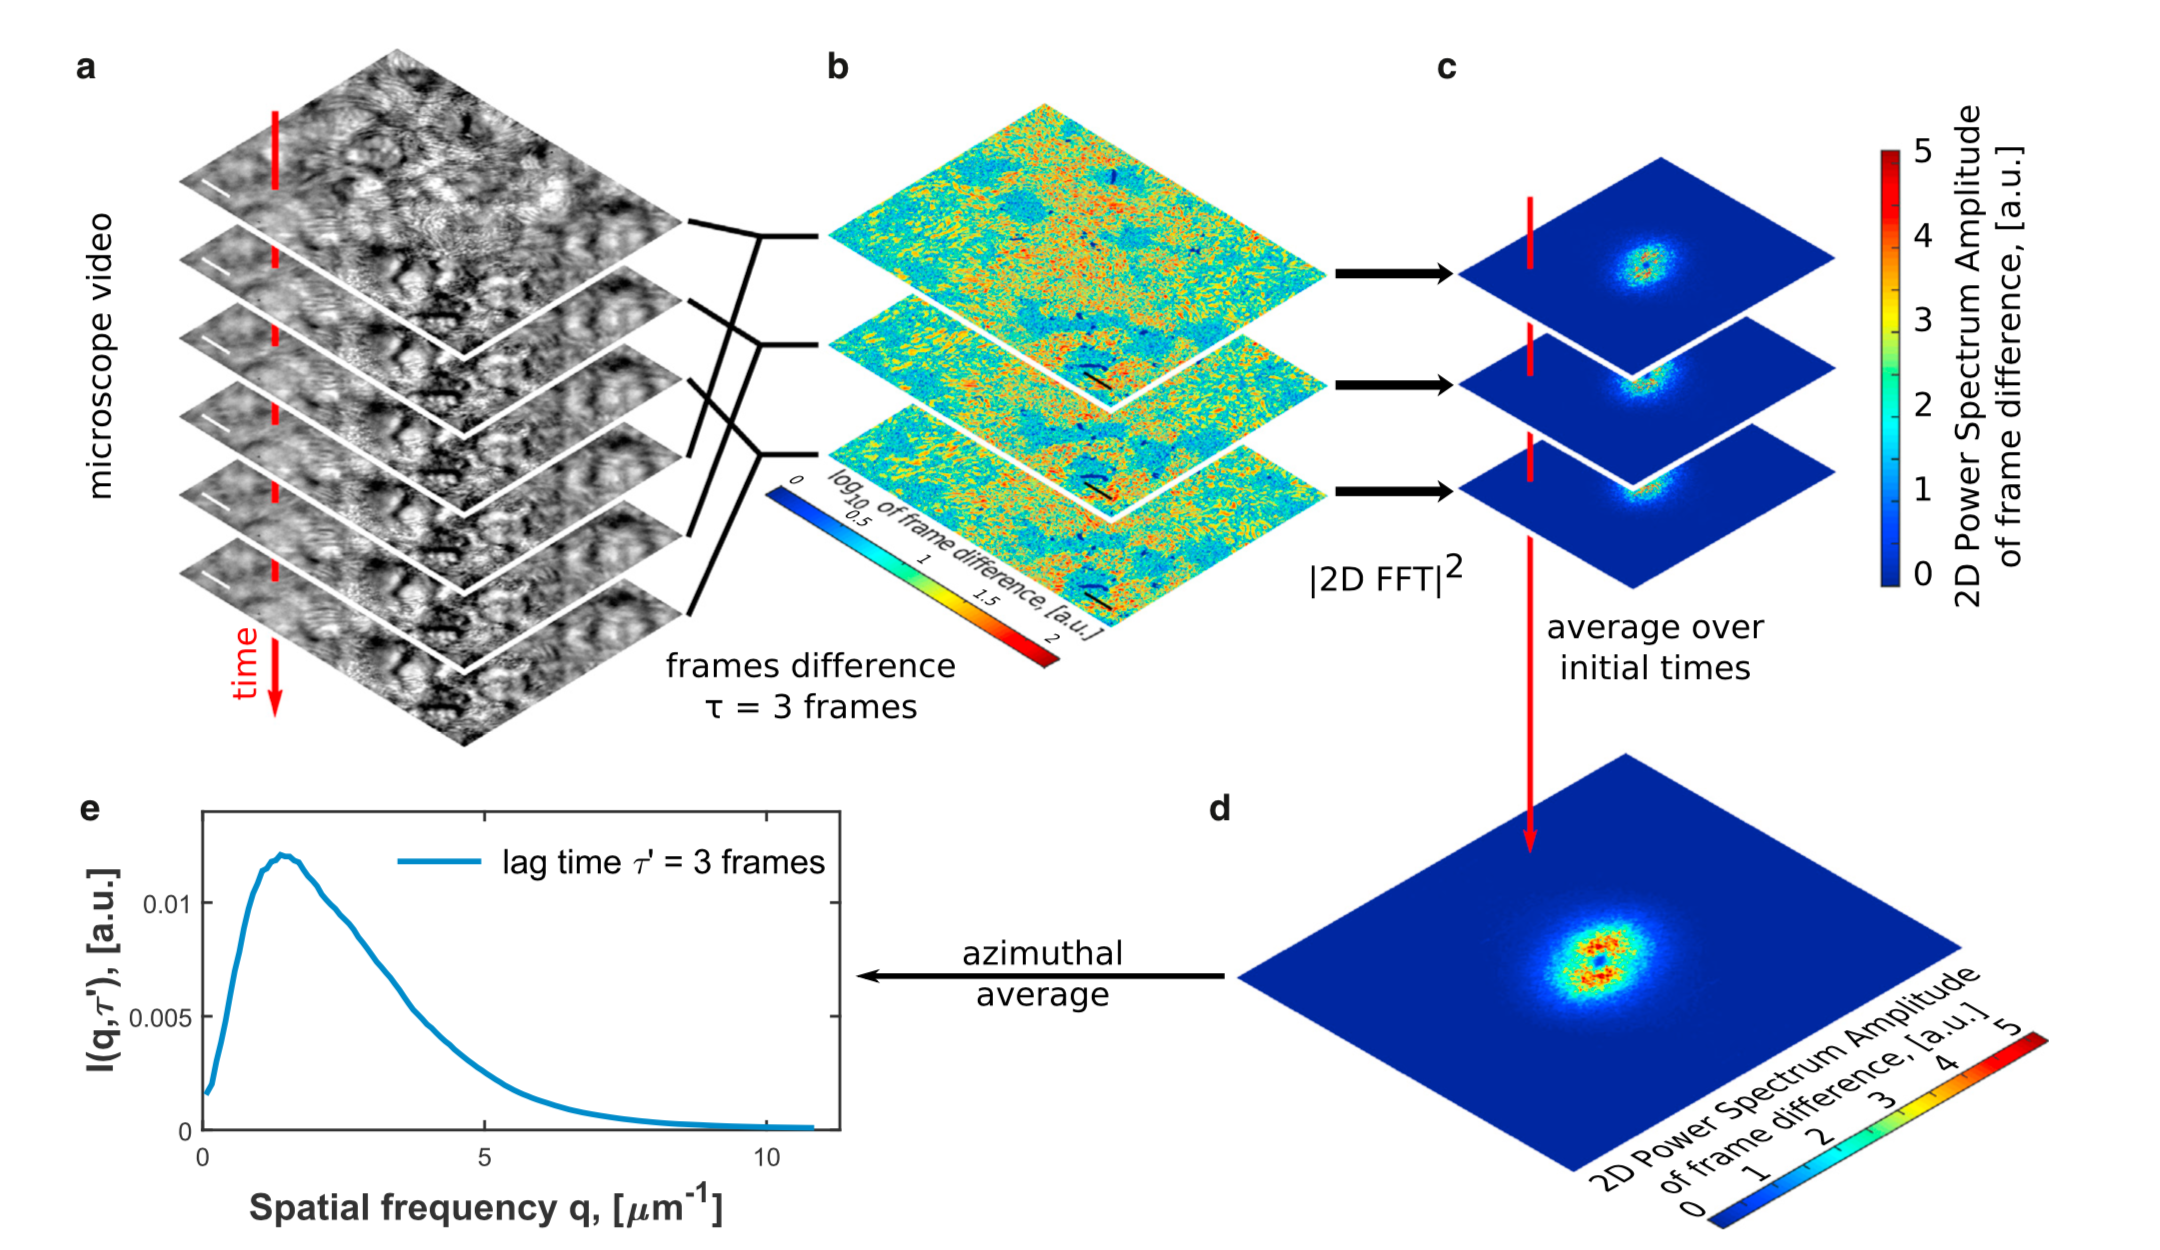
\includegraphics[height=5.5cm]{images/ddmpic.png}
\caption{Provides an overview of the DDM method as applied to the analysis of collective dynamics in ciliated cells.\cite{ddm2}}
\end{figure}

\begin{enumerate}[label=\alph*]
\item we take a video of the motion we wish to analyse and convert each frame into a 2D array of gray-scale pixel intensities.
\item for each starting frame in the video we take the difference between the pixel intensities of that frame and all lagging frames. $ \tau $ 
denotes the temporal separation of the two frames ( $ \tau = 3 $ frames,  is shown for various start times $ t_0 $). We denote each of these differences $ d(\underline{x}, t_0, \tau) $.
\item the 2D spatial Fourier transform of $ d(\underline{x}, t_0, \tau) $ is then taken for all combinations of $ t_0 $ and $ \tau $. Giving us d as a function of wave-vector instead of position. $ d(\underline{q}, t_0, \tau) $. We then take the the modulus squared of each Fourier transform giving us a power spectrum $I(\underline{q}, t_0, \tau) = |d(\underline{q}, t_0, \tau)|^2$.
\item because the system is stationary (power spectrum should be independent of $t_0$ and should only depend on $\tau$) we therefore take the average of the Fourier transforms over each $t_0$. This allows us to remove the dependence of $t_0$ from I and also reduce the effects of experimental uncertainty.
\item in the current case the system is also isotropic and so we can then take the azimuthal average of the 2D power spectrum. This means the power spectrum is now only a function of the modulus of the wave-vector q. $I(q, \tau)$
\item the expected functional form (for Brownian Motion) of this power spectrum has been proven to be $I(q, \tau) = A(q) \cdot (1 - e^{-\tau / \tau_c (q)}) + B(q)$ \cite{DLSPecora}. The physically interesting information is contained within $\tau_c$. $\tau_c$ for Brownian motion has been shown to equal $(D \cdot q^2)^{-1}$. Fitting the data (at each $\tau$) to this functional form and then extracting the value of $\tau_c$ as a function of q will yield the diffusion coefficient D. Plotting $log(\tau_c)$ against $log(q)$ should show a relationship of the form $y = -2\cdot x - log(D)$. The diffusion coefficient can then be used to find other pieces of information about the system including the size of the colloidal particles as there is a known relationship $D=\frac{k_B T}{6 \pi \eta R}$ between these two variables \cite{wynot_2002}.
\end{enumerate}

\subsection{Types of Crowd}
In this project we will be focusing primarily on two types of crowd. Crowds which are "stationary" for example people sat inside a stadium. Motion is restricted to oscillations around the person's average location. We term this crowd type "Brownian-like". The other type is that where the crowd shows some overall direction of travel. For example runner's in a marathon. We term this type of crowd "Swimmer-like". Videos have been typecast in to one of these two categories or neither (if they show a different type of motion). We expect the ISF for videos of a particular category to be similar (albeit with different values for the fit parameters) i.e of the same functional form. For the Brownian-like crowds we will try a fit of the type expected for Brownian motion (equation [7]). And for Swimmer-like crowds we will try a fit of the expected type for ballistic motion (equation [9]).

\clearpage
\section{Implementation}

DDM is a very computationally intensive algorithm, in order to approach real-time speeds it was necessary to focus on producing an optimal implementation from the start. Certain design decisions were primarily made in order to facilitate the required optimisations. The design decisions and how they were made will be explained in the following paragraph. An outline of the algorithm pipeline will then complete this section.
\\\\
Because of the nature of the DDM algorithm (mainly large array manipulations) it was decided that the code should target GPUs due to their suitability for highly parallelised array based Mathematics. An Nvidia Jetson TX2 was provided as a development board (will now be referred to as just the Jetson). The Jetson is a powerful, energy efficient development board with an embedded GPU\cite{jetson}. The Jetson GPU can be coded with the programming language CUDA, but after carrying out initial research \cite{cuda_book} it was decided that writing raw CUDA code by hand would be a significant undertaking and so other avenues to utilise GPU parallelism were explored. After careful consideration the library ArrayFire was selected as it offered optimised algorithms for several backends (GPU: CUDA/OPENCL and CPU: All)\cite{arrayfire}. This was an important feature as it meant it would be possible to avoid timely reimplementations of various algorithms and also that rapid prototyping on any development machine was possible due to the available CPU and OPENCL backends.
\\\\
Due to the selection of Arrayfire (availability of language bindings), the focus on speed and my own programming knowledge the selection of programming language was effectively limited to C++ or Rust\cite{rust} (for core algorithm implementation). Rust is a relatively recently developed programming language with a focus on speed, safety and concurrency. I selected Rust for the core of the algorithm implementation as it allows you to develop concurrent code in a much easier and safer way than C++, this is important so that the algorithm will not be bound by the CPU (passing data around, reading frames, sequential operations). Due to the relative immaturity of Rust language bindings for popular libraries are still in their infancy. This required me to create a small C++ library to expose language bindings for OpenCV over a C ffi (foreign function interface). OpenCV is used to capture video streams from files, cameras, urls etc. Frames from these streams are then sent into the DDM algorithm as they become available. This level of optimisation allows the bulk of the algorithm to run in less time than the length of the video (even using the CPU backend). There however is a significant slowdown associated with the radial averaging of the Fourier Transforms during the DDM algorithm. This slowdown prevents the algorithm from running in real-time but with further development it is anticipated that radial averaging can be optimised as the algorithm used currently only uses very rudimentary techniques (time limitations have so far prevented the implementations of these optimisations). After completion of the DDM algorithms the raw data is added to an SQlite database to allow efficient querying of the available data.
\\\\
Again due to time limitations and the immaturity of the Rust library ecosystem all data analysis (image structure function fitting etc. The ISFs are often not linearisable which means we have to resort to non-linear least-squares regression, scipy provides built in methods for this based on the Levenberg-Marquardt  algorithm\cite{scipy_fit}.) and data exploration was undertaken using Python (numpy, scipy, matplotlib, pandas, sqlite, etc.) and Jupyter Notebooks. If time permitted a custom curve fitting solution would have been added to the Rust codebase so that the algorithm could run as a totally self contained executable. This custom fitting solution would need to be implemented if DDM were to find an application in real-time autonomous crowd monitoring systems.
\\\\
Software development best practices were followed throughout development. The project was version controlled using Git, continuously integrated using TravisCI and a custom docker image, the set-up of both a mac OS and Linux based development environment was documented in detail, and core algorithms were benchmarked and tested in depth.
\\\\
\subsection{Algorithm Pipeline}
\begin{figure}[H]
%algorithm pipeline	
\centering
\noindent \includegraphics[height=0.7\paperwidth, width=0.6\paperwidth]{images/algo-pipeline.png}
\caption{Flow chart of the algorithm structure used in this project.}
\end{figure}
 
\clearpage
\section{Results}
%TODO: All multi-ddm and analyse

\clearpage
\section{Discussion}

\clearpage
\section{Future}
%TODO: Monday Tuesday 22-23/04/2019
\subsection{Comparisons}
\subsection{Advantages}
\subsection{Disadvantages}
\subsection{Applications}
\subsection{Further Development}

\clearpage
\section{Conclusion}


\clearpage
\section{References}
\printbibliography[heading=none]

\clearpage
\section{Appendices}
\subsection{Code}

\end{document}
